\chapter{Marco teórico}
\label{ch:marco-teorico}
Este capítulo reúne los fundamentos necesarios para comprender la adaptación de modelos de lenguaje mediante entrenamiento supervisado y aprendizaje por refuerzo. El recorrido comienza con la adaptación de dominio y el post training, desarrolla las señales de aprendizaje y los algoritmos PPO y GRPO, y presenta después las rúbricas, los modelos jueces y la evaluación externa. Las configuraciones de los experimentos se describen junto con su aplicación y sus resultados.

\section{Adaptación de dominio y post training}
\label{sec:marco-post-training}
Durante el preentrenamiento, un modelo de lenguaje desarrolla capacidades generales a partir de grandes corpus, mientras que la adaptación de dominio busca orientar esas capacidades hacia el vocabulario, los conocimientos y las tareas de un ámbito específico. En este contexto, el proceso de post training puede combinar demostraciones supervisadas con la evaluación de respuestas generadas por el propio modelo, de modo que cada etapa aporta una señal de aprendizaje diferente~\cite{gururangan2020dontstop,ouyang2022instructgpt}.

Dentro de las estrategias de adaptación, el preentrenamiento adaptativo al dominio (DAPT) continúa el aprendizaje sobre textos especializados, mientras que la adaptación al corpus de una tarea (TAPT) utiliza textos asociados a esa tarea~\cite{gururangan2020dontstop}. Por su parte, el SFT utiliza demostraciones explícitas de cómo responder, de manera que incorporar documentos del área y entrenar con pares de consulta y respuesta no constituye el mismo procedimiento. En consecuencia, su alcance depende de la calidad y la cobertura de las referencias, cuyos errores u omisiones también pueden aprenderse.

La elección de la señal depende también de la tarea. En problemas con resultados verificables puede utilizarse una regla que compruebe la solución, mientras que en dominios abiertos algunos aspectos admiten comprobaciones automáticas y otros requieren interpretar el contenido y el contexto~\cite{deepseek2025r1,arora2025healthbench}. Esta diferencia motiva estudiar cómo construir recompensas a partir de criterios explícitos, después de establecer los fundamentos del ajuste supervisado y del aprendizaje por refuerzo.
%
\section{Ajuste fino supervisado}
\label{sec:marco-sft}
\subsection{Objetivo y funcionamiento del ajuste fino supervisado}
\label{sec:sft-objetivo}
El ajuste fino supervisado, conocido como Supervised Fine-Tuning (SFT), utiliza demostraciones para orientar un modelo hacia una tarea, un formato de interacción o un dominio. Su punto de partida son parámetros obtenidos durante el preentrenamiento, que se ajustan con un conjunto de ejemplos de entrada y respuesta~\cite{ouyang2022instructgpt}, representado como
\begin{equation}
\mathcal{D}_{\mathrm{SFT}}=\{(x_i,y_i)\}_{i=1}^{N},
\label{eq:datos-sft}
\end{equation}
donde $x_i$ reúne la instrucción, la consulta y el contexto disponible, $y_i$ es la respuesta de referencia y $N$ indica la cantidad de ejemplos. El entrenamiento busca aumentar la probabilidad de esas respuestas condicionadas a sus entradas, por lo que las demostraciones determinan qué contenido y qué formas de respuesta se favorecen.


%
\subsection{Preparación de ejemplos y predicción autorregresiva}
\label{sec:sft-ejemplos}
Antes de entrenar, cada ejemplo se transforma en una secuencia de tokens mediante el tokenizador del modelo. En un formato conversacional, una plantilla organiza las instrucciones y los mensajes e incorpora delimitadores de roles, por lo que deben respetarse las convenciones del modelo de partida. Si $T_i$ es la longitud de la respuesta $i$, su probabilidad se descompone en predicciones del token siguiente,
\begin{equation}
p_\theta(y_i\mid x_i)=\prod_{t=1}^{T_i}
p_\theta(y_{i,t}\mid x_i,y_{i,<t}),
\label{eq:sft-autorregresivo}
\end{equation}
donde $\theta$ representa los parámetros del modelo y $y_{i,<t}$ contiene los tokens anteriores de la respuesta. Esta distribución es la que, en la sección~\ref{sec:marco-rl}, se interpretará como política y se denotará por $\pi_\theta$.

Durante el entrenamiento se aplica teacher forcing, una técnica que utiliza los tokens anteriores de la respuesta de referencia como contexto para predecir el siguiente token. En cada posición, el modelo recibe la consulta y la parte de la referencia que precede al token esperado, y la pérdida compara la distribución que produce con ese token correcto. Así, aunque asigne mayor probabilidad a un token incorrecto, las predicciones siguientes siguen utilizando el historial de la referencia. En cambio, durante la generación, el contexto se amplía con los tokens que el propio modelo va produciendo, de modo que un error puede influir en las predicciones posteriores.

Como la referencia completa está disponible durante el entrenamiento, un Transformer causal puede calcular las predicciones de distintas posiciones en paralelo, utilizando una máscara de atención que impide acceder a los tokens futuros~\cite{vaswani2017attention}. La figura~\ref{fig:sft-secuencia} muestra cómo se organizan el contexto, la respuesta y el relleno, distinguiendo qué información utiliza el modelo de qué posiciones se supervisan.

\begin{figure}[htbp]
\centering
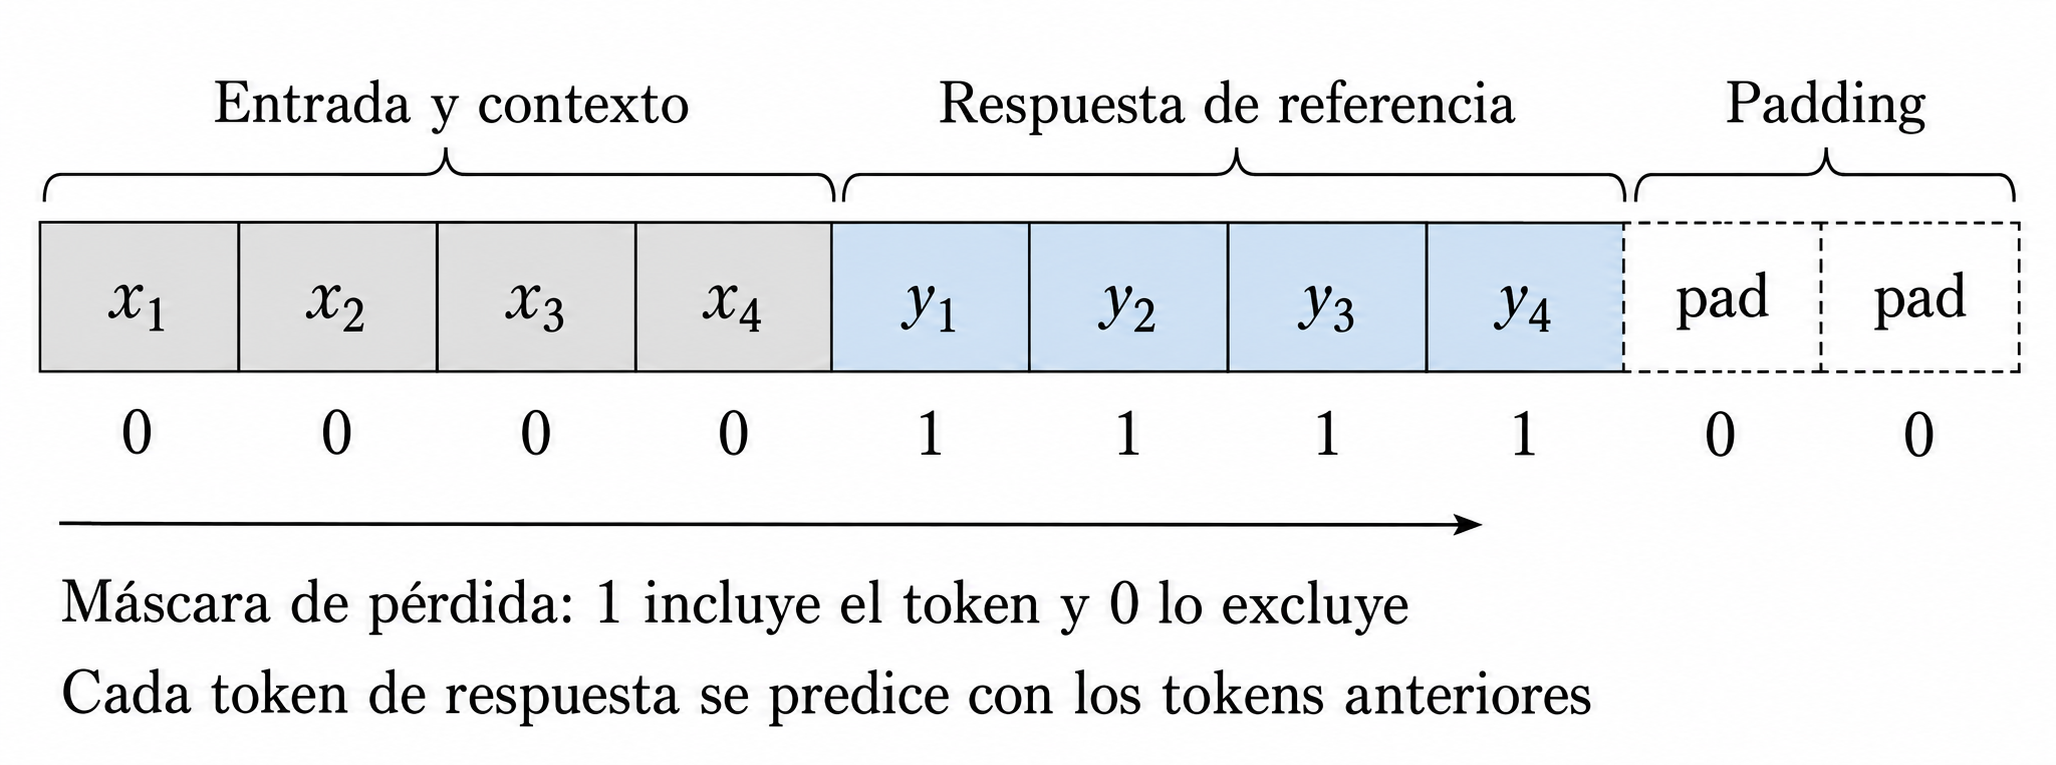
\includegraphics[width=0.95\textwidth]{Figuras/02-marco-teorico/02-ajuste-supervisado/sft-secuencia-tokens.png}
\caption{Secuencia de tokens con pérdida calculada únicamente sobre la respuesta.}
\label{fig:sft-secuencia}
\end{figure}

La preparación también requiere separar entrenamiento y validación, comprobar duplicados y evitar que una misma consulta o una variante cercana aparezca en ambos conjuntos. Asimismo, el límite de secuencia comprende la entrada y la respuesta, por lo que el truncamiento puede eliminar contexto o contenido supervisado y debe registrarse como parte del procedimiento. Este límite difiere de la cantidad máxima de tokens nuevos que se permite generar durante la inferencia, mientras que el padding permite reunir secuencias de longitudes distintas en un batch y se excluye de la pérdida para que el relleno no se aprenda como respuesta.

%
\subsection{Función de pérdida y actualización de parámetros}
\label{sec:sft-actualizacion}
Para el caso en que se supervisan únicamente los tokens de respuesta, la función de pérdida puede escribirse como el logaritmo de verosimilitud negativo promediado sobre esos tokens,
\begin{equation}
\mathcal{L}_{\mathrm{SFT}}(\theta)=
-\frac{1}{\sum_{i=1}^{N}T_i}
\sum_{i=1}^{N}\sum_{t=1}^{T_i}
\log p_\theta(y_{i,t}\mid x_i,y_{i,<t}).
\label{eq:sft}
\end{equation}
Esta expresión corresponde a una entropía cruzada con el token de referencia como etiqueta y penaliza que el modelo le asigne una probabilidad baja. En esta formulación, el promedio por tokens hace que una respuesta más larga aporte más términos al conjunto, por lo que no equivale a promediar primero la pérdida de cada respuesta y luego dar el mismo peso a todos los ejemplos. La maximización de probabilidades condicionales constituye el objetivo supervisado, independientemente de qué parámetros se permitan modificar~\cite{hu2022lora}.

Para expresar explícitamente la selección de posiciones, sea $z_i$ la secuencia completa del ejemplo y $m_{i,t}\in\{0,1\}$ una máscara que indica si el token en la posición $t$ contribuye a la pérdida. Entonces,
\begin{equation}
\mathcal{L}_{\mathrm{SFT}}(\theta)=
-\frac{\sum_{i,t}m_{i,t}\log p_\theta(z_{i,t}\mid z_{i,<t})}
{\sum_{i,t}m_{i,t}},
\label{eq:sft-mascara}
\end{equation}
siempre que exista al menos un token supervisado. En el ejemplo de la figura \ref{fig:sft-secuencia}, la máscara vale uno en la respuesta y cero en el contexto y el padding. Esta máscara de pérdida cumple una función distinta de la máscara causal de atención, ya que un token excluido como objetivo puede seguir proporcionando contexto a las predicciones siguientes.

El entrenamiento procesa un batch, calcula las probabilidades y la pérdida, obtiene sus gradientes por retropropagación y aplica una actualización sobre el subconjunto entrenable $\theta_{\mathrm{train}}$. Una representación básica mediante descenso de gradiente es
\begin{equation}
\theta_{\mathrm{train}}\leftarrow\theta_{\mathrm{train}}
-\eta\,\nabla_{\theta_{\mathrm{train}}}\mathcal{L}_{\mathrm{SFT}},
\label{eq:sft-actualizacion}
\end{equation}
donde $\eta$ es la tasa de aprendizaje. Esta expresión explica la dirección de la actualización, aunque optimizadores como AdamW utilizan además estimaciones de momentos del gradiente y decaimiento de pesos separado de la actualización adaptativa, por lo que su operación no se reduce a ese paso básico~\cite{loshchilov2019adamw}.

El microbatch determina cuántos ejemplos se procesan simultáneamente, mientras que la acumulación de gradientes combina varias operaciones antes de actualizar los parámetros y permite aumentar el batch efectivo bajo restricciones de memoria. Por otra parte, una época corresponde a un recorrido por el conjunto de entrenamiento y la tasa de aprendizaje controla la escala de los cambios, por lo que estas decisiones deben interpretarse junto con la pérdida de validación, cuyo descenso indica un mejor ajuste a las referencias de ese conjunto.

%
\subsection{Entrenamiento de parámetros mediante LoRA}
\label{sec:sft-parametros}
El ajuste completo requiere calcular y almacenar gradientes y estados del optimizador para todos los parámetros del modelo, lo que aumenta el uso de memoria y el costo del entrenamiento. El ajuste parcial reduce esa carga al actualizar solo un subconjunto, aunque la adaptación queda condicionada por las capas o los módulos seleccionados. Frente a estas restricciones, LoRA incorpora matrices entrenables de rango reducido en las proyecciones elegidas y mantiene congelados sus pesos originales~\cite{hu2022lora}.

Como muestra la figura~\ref{fig:sft-parametros}, una misma entrada recorre dos ramas: la transformación original y la actualización de LoRA. Sus salidas se suman, de modo que el modelo puede modificar su respuesta mediante los parámetros añadidos sin actualizar la matriz base.

\begin{figure}[htbp]
\centering
\begingroup
\singlespacing
\definecolor{loratrain}{HTML}{286B9B}
\definecolor{lorafixed}{HTML}{87929A}
\begin{tikzpicture}[>=Stealth,
  block/.style={draw,line width=0.8pt,rounded corners=3pt,align=center,
    minimum height=1.0cm,minimum width=1.8cm,inner sep=6pt,font=\small},
  train/.style={draw=loratrain,fill=loratrain!9},
  fixed/.style={draw=lorafixed,fill=lorafixed!12},
  flow/.style={->,line width=0.85pt,draw=black!65}]
\node[font=\normalsize] (input) at (0,0) {$x$};
\coordinate (split) at (0.7,0);
\node[block,fixed,minimum width=2.5cm] (base) at (3.3,1.25) {$W_0$\\Congelada};
\node[block,train] (a) at (2.0,-1.2) {$A$\\Entrenable};
\node[block,train] (b) at (4.5,-1.2) {$B$\\Entrenable};
\node[block,minimum width=1.0cm,draw=black!45] (scale) at (6.7,-1.2) {$\alpha/r$};
\node[circle,draw=black!60,minimum size=7mm,inner sep=0pt] (sum) at (8.3,1.25) {$+$};
\node[font=\normalsize] (output) at (9.4,1.25) {$y$};
\draw[draw=black!65,line width=0.85pt] (input) -- (split);
\fill[black!65] (split) circle (1.3pt);
\draw[flow,draw=lorafixed] (split) |- (base.west);
\draw[flow,draw=lorafixed] (base) -- (sum);
\draw[flow,draw=loratrain] (split) |- (a.west);
\draw[flow,draw=loratrain] (a) -- (b);
\draw[flow,draw=loratrain] (b) -- (scale);
\draw[flow,draw=loratrain] (scale.east) -| (sum.south);
\draw[flow] (sum) -- (output);
\node[font=\small,align=center] at (4.7,-2.6)
  {$y=W_0x+\dfrac{\alpha}{r}BAx$};
\end{tikzpicture}
\endgroup

\caption{LoRA: pesos base congelados y matrices $A$ y $B$ entrenables.}
\label{fig:sft-parametros}
\end{figure}

Para una matriz $W_0\in\mathbb{R}^{d_{\mathrm{out}}\times d_{\mathrm{in}}}$, la transformación utiliza los pesos efectivos
\begin{equation}
W_{\mathrm{eff}}=W_0+\frac{\alpha}{r}BA,
\qquad A\in\mathbb{R}^{r\times d_{\mathrm{in}}},
\qquad B\in\mathbb{R}^{d_{\mathrm{out}}\times r},
\label{eq:sft-lora}
\end{equation}
donde $r$ determina el rango de la actualización y $\alpha/r$ controla su escala. La matriz $A$ proyecta la entrada a una dimensión reducida y $B$ la lleva a la dimensión de salida, mientras $W_0$ permanece fija.

Durante el SFT, la pérdida se calcula sobre las predicciones obtenidas con esta transformación. A continuación, la retropropagación calcula los gradientes de $A$ y $B$, y el optimizador actualiza esas matrices para reducir la pérdida. Los pesos de $W_0$ siguen interviniendo en el cálculo de la salida, pero no reciben actualizaciones. Este procedimiento se aplica a cada proyección seleccionada para incorporar LoRA.

Para esa matriz, la cantidad de parámetros entrenables añadidos es
\begin{equation}
P_{\mathrm{LoRA}}=r(d_{\mathrm{in}}+d_{\mathrm{out}}),
\qquad P_{W_0}=d_{\mathrm{in}}d_{\mathrm{out}},
\label{eq:sft-lora-parametros}
\end{equation}
por lo que un rango pequeño reduce el número de parámetros entrenables y los recursos necesarios para calcular y almacenar sus gradientes y estados del optimizador, disminuyendo así el costo del entrenamiento. La selección de proyecciones, el rango y la escala definen la configuración de los adaptadores.
%
%
\section{Aprendizaje por refuerzo y recompensas verificables}
\label{sec:marco-rl}
En el aprendizaje por refuerzo, la señal procede de evaluar las respuestas que genera el modelo. Para comprender su relación con el SFT, primero se describe la generación de texto como una secuencia de decisiones y después se examinan las fuentes de recompensa.

\subsection{Fundamentos del aprendizaje por refuerzo aplicado al lenguaje}
\label{sec:rl-lenguaje}
El aprendizaje por refuerzo estudia cómo un agente modifica su comportamiento a partir de las consecuencias de sus acciones al interactuar con un entorno, buscando maximizar la recompensa acumulada esperada~\cite{sutton2018reinforcement}. Para elegir una acción, el agente utiliza una política que relaciona el estado disponible con las acciones posibles, mientras que el entorno determina la transición al estado siguiente y las señales de recompensa. De este modo, el aprendizaje depende tanto de las decisiones tomadas como de la evaluación de sus consecuencias, que puede recibirse inmediatamente o después de varias acciones.

En la generación de texto, el modelo de lenguaje actúa como agente y su distribución de probabilidades constituye la política, representada por $\pi_\theta$, donde $\theta$ reúne los parámetros entrenables. Si $x$ es la consulta y $y_{<t}$ contiene los tokens ya generados, el estado en el paso $t$ puede escribirse como $s_t=(x,y_{<t})$, mientras que la acción consiste en seleccionar el token siguiente $y_t$. Por lo tanto, cada elección amplía el contexto disponible para la próxima, y la sucesión de acciones forma una trayectoria que termina cuando se genera el token de fin o se alcanza el límite de longitud. En este caso, el entorno comprende el procedimiento que actualiza el contexto y el mecanismo que evalúa la respuesta, sin que sea necesario interactuar con un paciente real para entrenar sobre consultas almacenadas~\cite{ouyang2022instructgpt}.

Cuando se asigna una recompensa al finalizar la respuesta, un objetivo simplificado consiste en aumentar su valor esperado sobre las consultas de entrenamiento,
\begin{equation}
J(\theta)=\mathbb{E}_{x\sim\mathcal{D},\,y\sim\pi_\theta(\cdot\mid x)}[R(x,y)],
\label{eq:objetivo-rl}
\end{equation}
donde $\mathcal{D}$ representa la distribución de consultas y $R(x,y)$ evalúa la respuesta generada. Esta expresión no incluye todavía las restricciones de estabilidad del algoritmo y tampoco exige una respuesta de referencia única, aunque una referencia puede intervenir en la evaluación. Además de recompensas finales, es posible introducir señales sobre pasos intermedios, lo que permite distinguir la evaluación del resultado de la evaluación del proceso seguido para obtenerlo~\cite{lightman2023verify}.

%
\subsection{Diferencias entre aprendizaje supervisado y aprendizaje por refuerzo}
\label{sec:sft-rl}
La diferencia entre ambos procedimientos se encuentra en la señal que orienta la actualización. En el ajuste fino supervisado, desarrollado en el sección~\ref{sec:marco-sft}, la respuesta de referencia determina los tokens que intervienen en la pérdida de la ecuación \ref{eq:sft}, mientras que en el entrenamiento por refuerzo se evalúan respuestas producidas por la propia política. Esa evaluación proporciona una señal de calidad, pero no necesariamente indica qué token debería haberse generado en cada posición, por lo que el algoritmo debe relacionarla con las probabilidades de las acciones tomadas~\cite{ouyang2022instructgpt}. La figura \ref{fig:sft-rl} permite comparar el origen de las respuestas y el cálculo utilizado para actualizar el modelo.

\begin{figure}[htbp]
\centering
\begingroup
\singlespacing
\begin{tikzpicture}[>=Stealth,
 box/.style={draw,rounded corners=2pt,align=center,text width=2.6cm,minimum height=1.3cm,font=\small},
 note/.style={align=left,font=\small}]
\node[note,anchor=west] at (-1.3,1.2) {\textbf{Ajuste fino supervisado (SFT)}};
\node[box] (s1) at (0,0) {Consulta y respuesta de referencia};
\node[box] (s2) at (3.35,0) {Probabilidades de los tokens de referencia};
\node[box] (s3) at (6.7,0) {Pérdida supervisada};
\node[box] (s4) at (10.05,0) {Actualización de parámetros};
\draw[->] (s1)--(s2); \draw[->] (s2)--(s3); \draw[->] (s3)--(s4);
\node[note,anchor=west] at (-1.3,-1.4) {\textbf{Aprendizaje por refuerzo (RL)}};
\node[box] (r1) at (0,-2.6) {Consulta y respuestas generadas};
\node[box] (r2) at (3.35,-2.6) {Evaluación y recompensa};
\node[box] (r3) at (6.7,-2.6) {Ventaja y objetivo de la política};
\node[box] (r4) at (10.05,-2.6) {Actualización de parámetros};
\draw[->] (r1)--(r2); \draw[->] (r2)--(r3); \draw[->] (r3)--(r4);
\end{tikzpicture}
\endgroup

\caption{Comparación entre el ajuste fino supervisado y el aprendizaje por refuerzo.}
\label{fig:sft-rl}
\end{figure}

Ambos procedimientos pueden combinarse cuando el SFT proporciona un comportamiento inicial adecuado y el refuerzo busca ajustar propiedades que la reproducción de demostraciones no controla de manera explícita. Sin embargo, esta secuencia es una decisión de diseño y no una condición general del aprendizaje por refuerzo, como muestra el entrenamiento de DeepSeek-R1-Zero directamente sobre un modelo base~\cite{deepseek2025r1}. La comparación entre SFT y RL debe considerar, por tanto, el punto de partida, los datos y la recompensa utilizados.

%
\subsection{Construcción de la señal de recompensa}
\label{sec:senal-recompensa}
La recompensa expresa qué comportamientos se busca favorecer y cuáles se intenta reducir, por lo que su construcción determina la dirección del entrenamiento. Una posibilidad es obtener evaluaciones humanas sobre respuestas generadas o comparaciones entre pares de respuestas, que permiten aprender un modelo de recompensa capaz de predecir preferencias~\cite{christiano2017preferences,ouyang2022instructgpt}. También puede utilizarse retroalimentación de otros modelos para construir esas preferencias o valorar las respuestas, como ocurre en los procedimientos de aprendizaje con feedback de inteligencia artificial~\cite{bai2022constitutional}. Estas fuentes no son equivalentes, ya que dependen de distintos evaluadores y pueden reproducir sus sesgos.

Cuando existe una condición comprobable, la recompensa puede obtenerse mediante un verificador programático que compare un resultado, ejecute pruebas sobre código o compruebe una restricción de formato~\cite{deepseek2025r1}. Este uso de condiciones comprobables corresponde al aprendizaje por refuerzo con recompensas verificables (RLVR). Una comprobación binaria asigna dos resultados posibles, mientras que una señal graduada permite distinguir niveles de desempeño. Asimismo, la evaluación puede referirse al resultado final o a pasos del razonamiento, una distinción que afecta a la información que recibe el entrenamiento~\cite{lightman2023verify}.

PPO y GRPO utilizan habitualmente una recompensa escalar para calcular la actualización, por lo que el procedimiento de evaluación debe producir un valor que permita comparar las respuestas. Además, el evaluador no necesita ser diferenciable, ya que en los métodos de gradiente de política la señal evaluativa se combina con las probabilidades de las acciones generadas por el modelo~\cite{sutton2018reinforcement}. Por ejemplo, para una recompensa final y una consulta fija, la identidad
\begin{equation}
\nabla_\theta\mathbb{E}_{y\sim\pi_\theta}[R(x,y)]
=\mathbb{E}_{y\sim\pi_\theta}
[R(x,y)\nabla_\theta\log\pi_\theta(y\mid x)]
\label{eq:gradiente-politica}
\end{equation}
muestra que, cuando $R$ se trata como una evaluación fija sin dependencia directa de $\theta$, el gradiente se calcula sobre la política y no atraviesa el juez. Esta relación fundamenta el uso de verificadores y evaluadores externos, aunque los algoritmos prácticos añaden estimadores de ventaja y mecanismos de estabilidad.

%
%
\section{Optimización mediante PPO y GRPO}
\label{sec:marco-optimizacion}
La recompensa orienta la actualización de la política al favorecer las respuestas mejor evaluadas, mientras que PPO y GRPO incorporan mecanismos para controlar esos cambios.

\subsection{Ciclo de optimización y mecanismos de estabilidad}
\label{sec:ciclo-optimizacion}
El ciclo de entrenamiento comienza al seleccionar consultas y generar respuestas mediante una política de muestreo, a partir de las cuales se calculan recompensas y ventajas para actualizar los parámetros. La ventaja indica qué tan favorable resulta una acción o respuesta respecto de una referencia de comparación, lo que permite distinguir una recompensa alta en términos absolutos de una respuesta mejor que las alternativas consideradas. Después de la actualización, se vuelve a generar con la política modificada y se repite el procedimiento, como se representa en la figura \ref{fig:ciclo-rl}~\cite{schulman2017ppo,shao2024deepseekmath}.

\begin{figure}[htbp]
\centering
\begingroup
\singlespacing
\begin{tikzpicture}[>=Stealth,
 box/.style={draw,rounded corners=2pt,align=center,text width=3.2cm,minimum height=1.1cm,font=\small},
 lbl/.style={font=\small,align=center}]
\node[box] (q) at (0,0) {Consultas del conjunto de entrenamiento};
\node[box] (p) at (4.5,0) {Política de recolección\\Generación de respuestas};
\node[box] (e) at (9,0) {Evaluador externo\\Cálculo de recompensas};
\node[box] (u) at (0,-2.5) {Política actual\\Actualización de parámetros};
\node[box] (a) at (4.5,-2.5) {Ventajas y probabilidades de los tokens};
\node[box,dashed] (ref) at (9,-2.5) {Política de referencia\\Comparación mediante KL};
\draw[->] (q)--(p); \draw[->] (p)--(e);
\draw[->] (e.south)--(9,-1.25)-|(a.north east);
\draw[->] (p.south)--(a.north);
\draw[->] (a)--(u);
\draw[->,dashed] (ref.south)--++(0,-0.6)-|(u.south);
\draw[->] (u.west)--(-2.2,-2.5)--(-2.2,1.35)--(4.5,1.35)--(p.north);
\node[lbl] at (4.1,1.95) {La política actualizada se usa en la siguiente iteración};
\end{tikzpicture}
\endgroup

\caption{Ciclo de generación, evaluación y actualización de la política.}
\label{fig:ciclo-rl}
\end{figure}

Para interpretar este ciclo conviene distinguir la política actual $\pi_\theta$, cuyos parámetros se optimizan, de la política de recolección $\pi_{\mathrm{old}}$, utilizada para generar el conjunto de respuestas de una iteración. Mientras se realizan actualizaciones sobre ese conjunto, ambas pueden diferir, por lo que el algoritmo compara las probabilidades de los tokens bajo las dos políticas. Por otra parte, la política de referencia $\pi_{\mathrm{ref}}$ puede mantenerse fija para regularizar la distancia respecto de un comportamiento inicial, y no debe confundirse con la política que produjo las respuestas de la iteración~\cite{shao2024deepseekmath}.

El muestreo permite obtener distintas respuestas para una misma consulta y, por ello, influye en las alternativas que el entrenamiento puede explorar. Sin embargo, aumentar la diversidad no garantiza que las respuestas sean útiles, mientras que una generación completamente determinista puede reducir la variación necesaria para comparar alternativas. Para controlar la actualización, algunos métodos utilizan clipping sobre la razón de probabilidades y una penalización por divergencia de Kullback y Leibler (KL). El primero limita el incentivo del objetivo a ciertos cambios respecto de la política de recolección, mientras que la segunda penaliza la distancia respecto de una política de referencia, por lo que cumplen funciones distintas y ninguno garantiza por sí solo la estabilidad del entrenamiento~\cite{schulman2017ppo,ouyang2022instructgpt}.

Para un estado fijo $s$, la divergencia KL entre la política actual y la de referencia se define como
\begin{equation}
D_{\mathrm{KL}}\!\left(\pi_\theta(\cdot\mid s)\,\|\,\pi_{\mathrm{ref}}(\cdot\mid s)\right)
=\sum_{a\in\mathcal{V}}\pi_\theta(a\mid s)
\log\frac{\pi_\theta(a\mid s)}{\pi_{\mathrm{ref}}(a\mid s)},
\label{eq:kl}
\end{equation}
donde $\mathcal{V}$ es el vocabulario de tokens y se supone que la política de referencia asigna probabilidad positiva a las acciones consideradas. Esta divergencia compara distribuciones completas y vale cero cuando coinciden, mientras que un coeficiente $\beta$ controla su contribución al objetivo. En implementaciones de entrenamiento puede estimarse mediante los tokens muestreados, por lo que también debe documentarse el estimador utilizado, además del valor de $\beta$~\cite{shao2024deepseekmath}.

%
\subsection{PPO como antecedente de la optimización de modelos de lenguaje}
\label{sec:ppo}
Proximal Policy Optimization (PPO) pertenece a los métodos de optimización de políticas y, en su formulación habitual de actor y crítico, combina una política que selecciona acciones con una función de valor que estima el retorno esperado desde un estado. Esta estimación ayuda a calcular las ventajas utilizadas para actualizar la política, mientras que el crítico se entrena a partir de los retornos observados. Para evitar que la reutilización de las muestras incentive cambios excesivos, una variante de PPO utiliza el objetivo con clipping~\cite{schulman2017ppo},
\begin{equation}
L^{\mathrm{clip}}(\theta)=\mathbb{E}_{t}\!\left[
\min\left(\rho_t(\theta)\widehat{A}_t,
\operatorname{clip}(\rho_t(\theta),1-\epsilon_c,1+\epsilon_c)\widehat{A}_t\right)
\right],
\label{eq:ppo}
\end{equation}
donde $\rho_t(\theta)=\pi_\theta(a_t\mid s_t)/\pi_{\mathrm{old}}(a_t\mid s_t)$ compara la probabilidad de la acción observada, $\widehat{A}_t$ es su ventaja estimada y $\epsilon_c$ determina el intervalo de recorte. De este modo, cuando el cambio de probabilidad ya favorece suficientemente una acción con ventaja positiva, el objetivo deja de premiar su aumento en la rama recortada, con un comportamiento análogo para acciones con ventaja negativa. Este mecanismo no impone una cota estricta a cada cambio de parámetros, sino que modifica el incentivo de optimización.

En InstructGPT, PPO se utilizó después del ajuste supervisado para optimizar las respuestas según un modelo de recompensa aprendido de preferencias humanas, incorporando además una regularización respecto de una política de referencia~\cite{ouyang2022instructgpt}. Su aplicación requiere obtener recompensas y estimaciones de valor, lo que añade cómputo y memoria al entrenamiento, aunque la cantidad de modelos almacenados y la posibilidad de compartir componentes dependen de la implementación. Este costo motivó alternativas como GRPO, que reemplaza el crítico aprendido por una comparación de recompensas dentro de cada grupo~\cite{shao2024deepseekmath}.

En este punto, conviene distinguir el algoritmo que actualiza la política del procedimiento que asigna la recompensa, ya que tanto PPO como GRPO pueden utilizar distintas señales de evaluación. Por lo tanto, el carácter verificable de RLVR depende de cómo se comprueba la respuesta y se obtiene esa señal, mientras que la diferencia entre ambos algoritmos reside aquí en cómo estiman las ventajas para orientar la actualización~\cite{schulman2017ppo,shao2024deepseekmath,deepseek2025r1}.
%
\subsection{GRPO y la optimización relativa por grupos}
\label{sec:grpo}
Group Relative Policy Optimization (GRPO) genera varias respuestas para una misma consulta y utiliza sus recompensas para estimar una ventaja relativa, evitando entrenar un crítico separado. Si el grupo contiene $G$ respuestas con recompensas $r_1,\ldots,r_G$, una expresión simplificada de esa ventaja es
\begin{equation}
A_i=\frac{r_i-\overline{r}}{\sigma_r+\varepsilon_n},
\qquad \overline{r}=\frac{1}{G}\sum_{i=1}^{G}r_i,
\qquad \sigma_r=\sqrt{\frac{1}{G}\sum_{i=1}^{G}(r_i-\overline{r})^2},
\label{eq:ventaja-grpo}
\end{equation}
donde $\overline{r}$ representa el promedio del grupo, $\sigma_r$ su dispersión y $\varepsilon_n$ un término pequeño de estabilidad numérica. La normalización por la media y la desviación estándar corresponde al mecanismo de la formulación original, mientras que el término añadido y la convención para calcular la desviación pueden variar entre implementaciones~\cite{shao2024deepseekmath}.

Una ventaja positiva favorece un aumento de la probabilidad de la respuesta respecto de la política de recolección, mientras que una negativa produce el incentivo contrario, sujeto al objetivo con clipping y a la regularización utilizada. Por lo tanto, importa la diferencia entre las recompensas y no solamente su promedio, ya que un grupo con recompensas idénticas tiene ventajas relativas nulas bajo la ecuación \ref{eq:ventaja-grpo}, aunque puedan existir gradientes de otros términos del objetivo. La figura \ref{fig:grpo-ejemplo} ilustra este cálculo con cuatro respuestas y valores elegidos únicamente para explicar el procedimiento.

\begin{figure}[htbp]
\centering
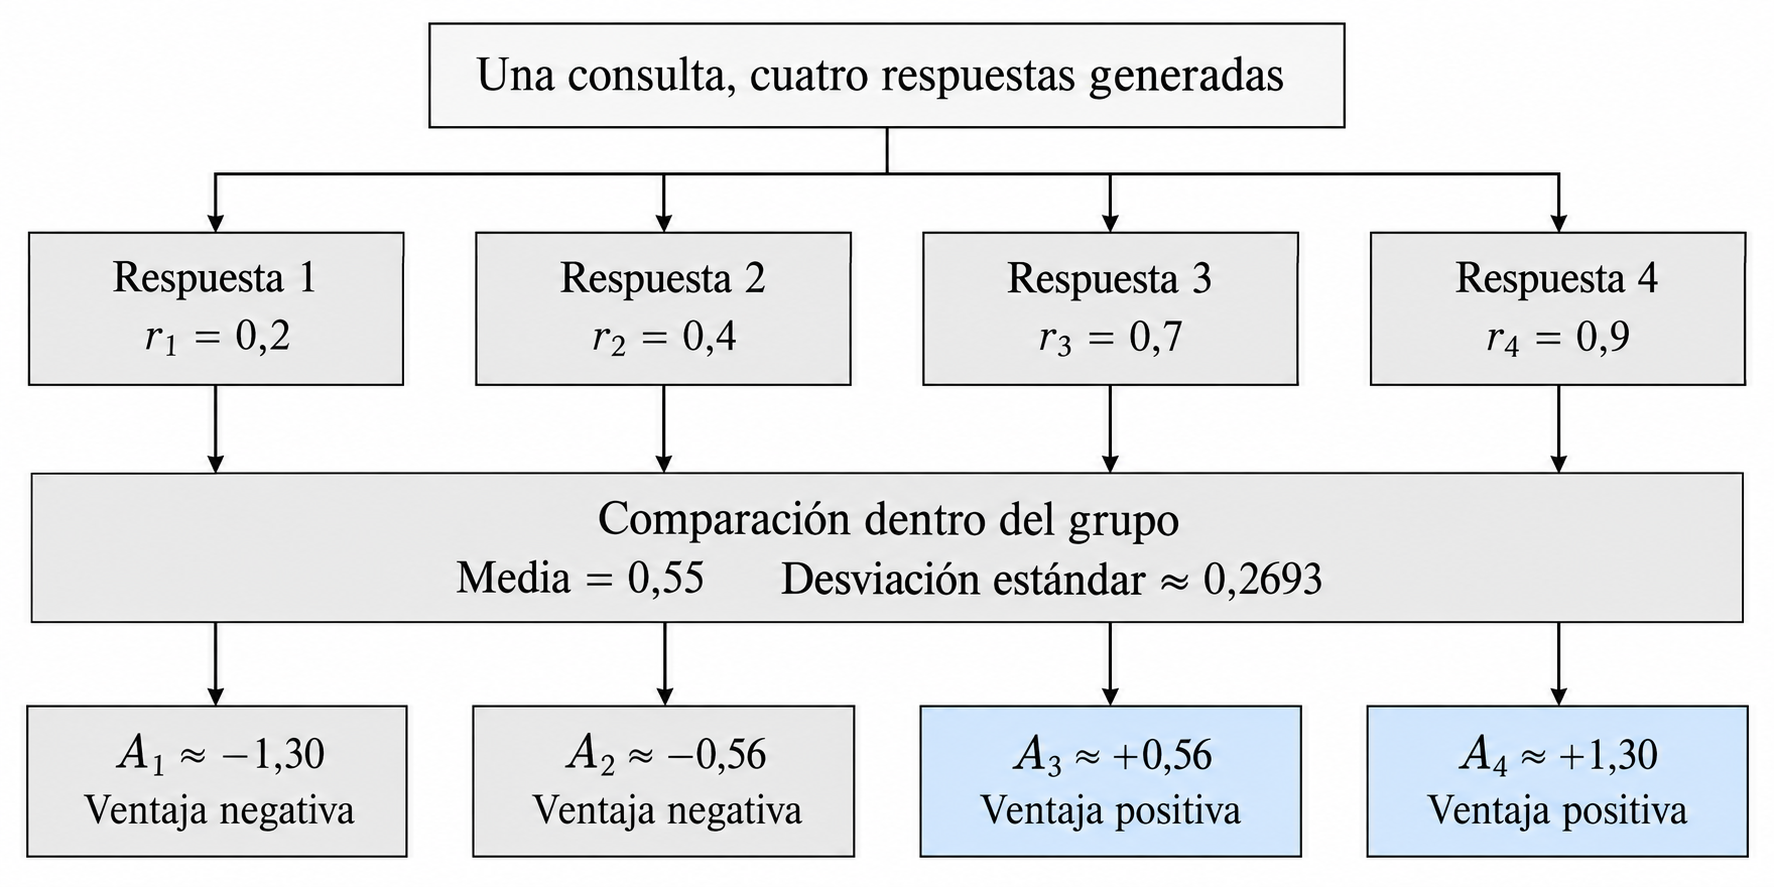
\includegraphics[width=0.95\textwidth]{Figuras/02-marco-teorico/04-ppo-grpo/rl-grpo-grupo.png}
\caption{Ejemplo ilustrativo de comparación de recompensas y ventajas en GRPO.}
\label{fig:grpo-ejemplo}
\end{figure}

Para relacionar esa comparación con la actualización de parámetros, puede escribirse el objetivo de GRPO con recompensa final como
\begin{equation}
\begin{aligned}
J_{\mathrm{GRPO}}(\theta)
&=\mathbb{E}_{x,\{y_i\}\sim\pi_{\mathrm{old}}}\left[
\frac{1}{G}\sum_{i=1}^{G}\frac{1}{T_i}\sum_{t=1}^{T_i}
\left(C_{i,t}(\theta)-\beta D_{i,t}(\theta)\right)\right],\\
C_{i,t}(\theta)
&=\min\left(\rho_{i,t}(\theta)A_i,
\operatorname{clip}(\rho_{i,t}(\theta),1-\epsilon_c,1+\epsilon_c)A_i\right),\\
\rho_{i,t}(\theta)
&=\frac{\pi_\theta(y_{i,t}\mid x,y_{i,<t})}
{\pi_{\mathrm{old}}(y_{i,t}\mid x,y_{i,<t})}.
\end{aligned}
\label{eq:objetivo-grpo}
\end{equation}
En esta expresión, las consultas se extraen de $\mathcal{D}$ y las respuestas se generan con la política de recolección, mientras que $T_i$ es la longitud de la respuesta $i$ y $D_{i,t}$ representa la divergencia respecto de la política de referencia en el contexto del token $t$. El término $C_{i,t}$ combina la razón de probabilidades con la ventaja y el recorte de PPO, mientras que $\beta D_{i,t}$ penaliza la desviación respecto de la referencia~\cite{shao2024deepseekmath}. Por lo tanto, maximizar este objetivo favorece los tokens de respuestas con mejor recompensa relativa, sujeto a esos mecanismos de control, y la pérdida utilizada para minimizar mediante descenso de gradiente puede definirse como $\mathcal{L}_{\mathrm{GRPO}}=-J_{\mathrm{GRPO}}$. La división por $T_i$ da el mismo peso total a cada respuesta antes de promediar el grupo, una elección que puede cambiar en otras variantes.

Cuando se utiliza una recompensa final, la ventaja de la respuesta puede aplicarse a sus tokens durante la actualización, aunque la formulación también contempla señales de proceso y variantes posteriores modifican la normalización y la ponderación por longitud~\cite{shao2024deepseekmath,deepseek2025r1}. En consecuencia, documentar que se utilizó GRPO no basta para reproducir una corrida, sino que deben precisarse su variante, la recompensa y las decisiones de implementación. Además, $G$ indica cuántas respuestas se generan por consulta y debe distinguirse del tamaño del microbatch y de la acumulación de gradientes, definidos en la sección \ref{sec:sft-actualizacion}.

%
%
\section{Rúbricas y modelos de lenguaje como jueces}
\label{sec:marco-rubricas}
En las tareas abiertas, una rúbrica descompone la evaluación en criterios que describen contenidos esperados, restricciones y errores relevantes. Cada criterio puede asociarse con un peso para combinar sus decisiones en una recompensa, permitiendo distinguir respuestas parcialmente satisfactorias. Rubicon estudia esta forma de supervisión en tareas abiertas, mientras que ARES genera preguntas, respuestas y rúbricas a partir de documentos~\cite{huang2025rubicon,li2026ares}.

Rubrics as Rewards (RaR) utiliza rúbricas específicas por consulta como señal de recompensa para entrenar mediante GRPO. Su construcción toma respuestas de referencia como fuente de supervisión y organiza los criterios para que puedan evaluarse individualmente. El trabajo estudia una agregación explícita, que combina decisiones de cumplimiento mediante sus pesos, y una agregación implícita, en la que el juez recibe la rúbrica y produce una puntuación global~\cite{gunjal2025rar}. Esta distinción permite estudiar por separado el contenido de los criterios y la forma en que sus evaluaciones se convierten en recompensa.

\subsection{Evaluación por criterios y ayudas durante la generación}
\label{sec:marco-jueces}
Un modelo de lenguaje puede actuar como juez al recibir la consulta, la respuesta generada y los criterios que debe comprobar. En una evaluación binaria por criterio, sus decisiones indican qué condiciones se cumplen y luego se agregan según sus pesos. A diferencia de una coincidencia literal, esta evaluación permite examinar formulaciones equivalentes, aunque su resultado depende de las instrucciones y de la interpretación del modelo evaluador~\cite{arora2025healthbench,zhou2026ruscarl}.

La rúbrica también puede intervenir en la generación al mostrar parte de sus criterios como ayudas. RuscaRL utiliza distintos niveles de asistencia y reduce su presencia durante el entrenamiento, manteniendo los criterios completos para evaluar las respuestas~\cite{zhou2026ruscarl}. Por ello, conviene distinguir la información visible para el modelo de la que utiliza el juez, así como la recompensa de entrenamiento de la evaluación externa.

\subsection{Limitaciones y evaluación del aprendizaje obtenido}
\label{sec:limites-rl}
La recompensa representa una aproximación al objetivo que se busca mejorar, por lo que maximizarla puede favorecer comportamientos que aprovechen errores del evaluador sin aumentar la calidad de las respuestas. Este fenómeno suele denominarse reward hacking, mientras que la sobreoptimización describe el deterioro que puede aparecer al optimizar excesivamente una señal imperfecta. Gao y sus colaboradores estudiaron esta divergencia mediante un entorno sintético con un modelo de recompensa de referencia y otro utilizado como aproximación, mostrando que el aumento de la señal optimizada puede coexistir con un deterioro de la evaluación de referencia~\cite{gao2022overoptimization}.

Para evaluar el aprendizaje obtenido se distingue la recompensa de entrenamiento del desempeño sobre consultas reservadas y de los resultados de un benchmark externo. La primera describe el ajuste a la señal utilizada, mientras que las otras permiten examinar si ese ajuste mejora las respuestas fuera del entrenamiento. Esta comparación requiere datos separados y protocolos consistentes, y debe complementarse con la revisión de errores que la recompensa puede pasar por alto. En el caso clínico, recuperar los conceptos esperados no basta para comprobar la pertinencia ni la seguridad de todas las recomendaciones, por lo que las rúbricas y las respuestas también requieren revisión experta.%
%
\section{Evaluación de la adaptación}
\label{sec:marco-evaluacion}
La evaluación externa examina las respuestas ante consultas distintas de las utilizadas para entrenar y permite estudiar si los cambios se mantienen fuera de la señal de recompensa. Su interpretación requiere identificar el benchmark, las condiciones de generación y el evaluador, además de definir cómo se agregan los criterios.

\subsection{HealthBench y evaluación por conversación}
\label{sec:marco-healthbench}
HealthBench es un benchmark desarrollado por OpenAI para evaluar respuestas médicas abiertas mediante criterios específicos de cada conversación, elaborados por profesionales médicos~\cite{arora2025healthbench}. Además de su versión general, el benchmark incluye las variantes HealthBench Hard y HealthBench Consensus, por lo que es necesario identificar de cuál procede cada evaluación.

El procedimiento conserva la conversación y su identificador, genera una respuesta al último mensaje del usuario y evalúa cada criterio a partir de esa respuesta y del contexto disponible. Las respuestas se guardan antes de calificarlas, mientras que las decisiones del juez y sus explicaciones se almacenan en archivos separados, lo que permite revisar una decisión individual o recalcular las métricas sin volver a generar el texto. Como muestra la figura \ref{fig:protocolo-evaluacion}, la rúbrica de HealthBench se proporciona únicamente al juez, de modo que el modelo evaluado responde sin acceder a esos criterios. Estas rúbricas pertenecen a la evaluación externa y deben distinguirse de las utilizadas como recompensa durante el entrenamiento.

\begin{figure}[htbp]
\centering
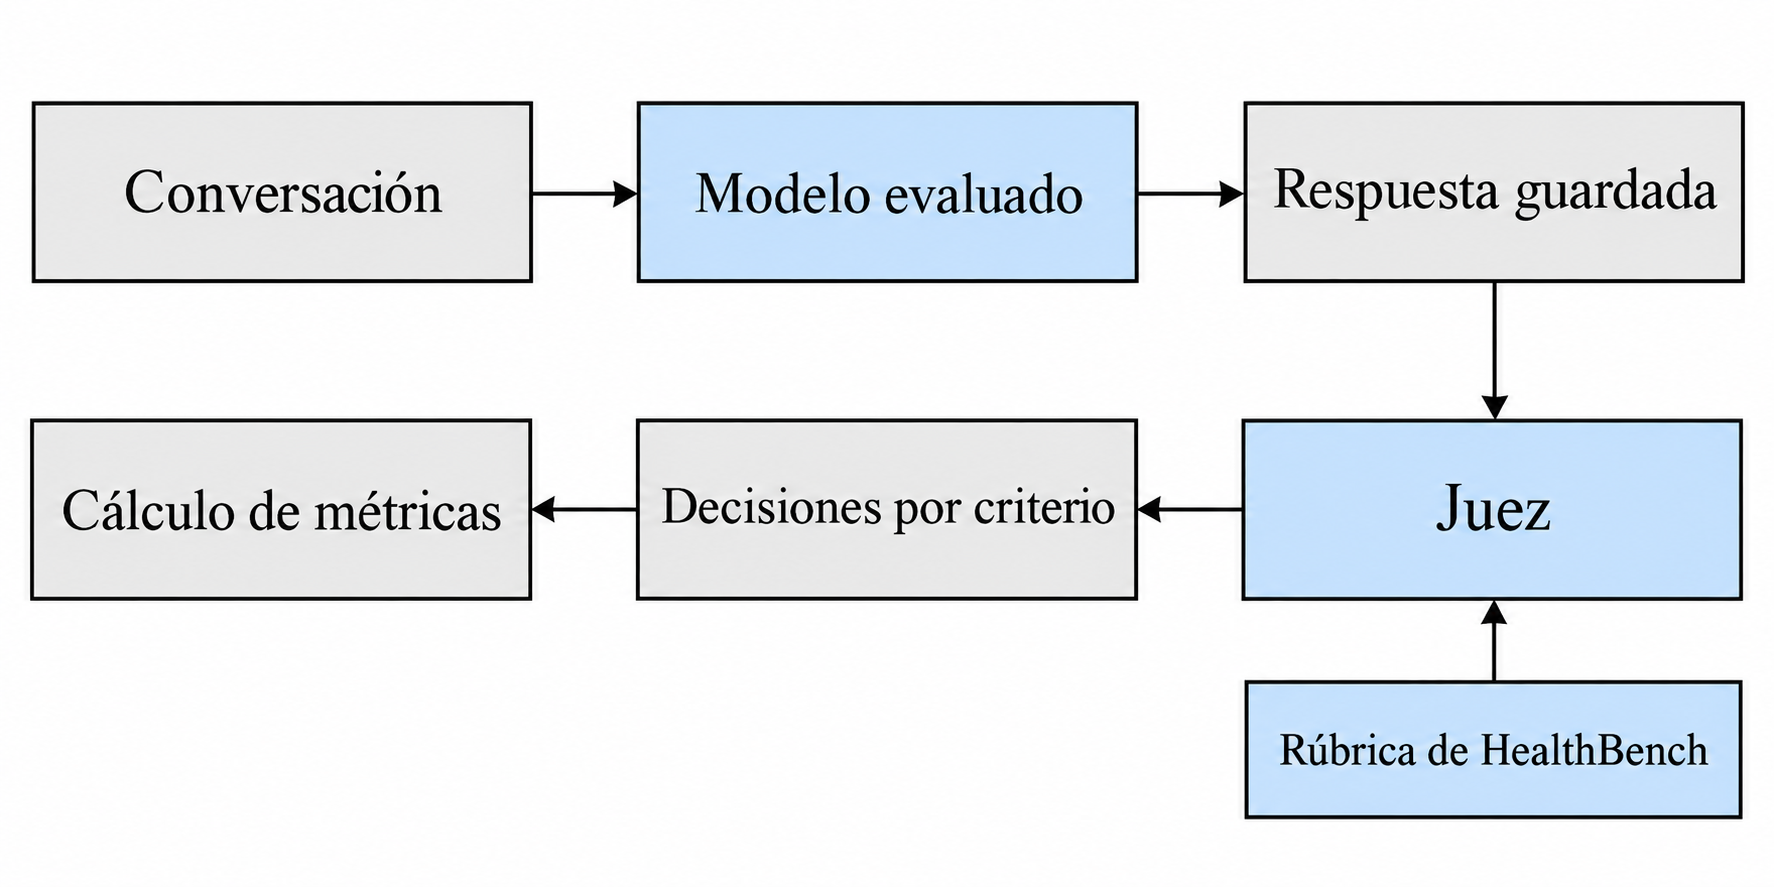
\includegraphics[width=0.95\textwidth]{Figuras/02-marco-teorico/06-evaluacion/evaluacion-protocolo.png}
\caption{Evaluación de respuestas mediante las rúbricas de HealthBench y un modelo juez.}
\label{fig:protocolo-evaluacion}
\end{figure}

Las condiciones concretas de la muestra, la generación y el juez del proyecto se describen en la sección~\ref{sec:protocolo-experimental}.

\subsection{Métricas y comparación de modelos}
\label{sec:evaluacion-metricas}
El puntaje principal combina los criterios cumplidos y sus pesos. Para el caso $i$, sea $p_{ij}$ el peso del criterio $j$ y $m_{ij}\in\{0,1\}$ la decisión de cumplimiento del juez. Si existen puntos positivos disponibles, el valor crudo del caso es
\begin{equation}
s_i=\frac{\sum_{j=1}^{M_i}p_{ij}m_{ij}}
{\sum_{j=1}^{M_i}\max(p_{ij},0)},
\label{eq:healthbench-caso}
\end{equation}
donde $M_i$ es la cantidad de criterios del caso. El numerador incorpora los puntos positivos obtenidos y las penalizaciones activadas, mientras que el denominador representa los puntos positivos disponibles. Por lo tanto, cumplir un criterio de peso negativo resta puntos y puede producir un valor individual negativo.

Para $N$ casos evaluados, el resultado global expresado en porcentaje se calcula como
\begin{equation}
S=100\,\operatorname{clip}\!\left(\overline{s},0,1\right),
\qquad \overline{s}=\frac{1}{N}\sum_{i=1}^{N}s_i.
\label{eq:healthbench-global}
\end{equation}
El orden de estas operaciones sigue el apéndice D de HealthBench y la implementación de simple-evals~\cite{arora2025healthbench,openai2026healthbenchcode}. Primero se promedian los valores crudos y después se recorta el promedio al intervalo indicado, por lo que recortar cada caso antes de promediar corresponde a otro cálculo. En consecuencia, en la formulación de HealthBench un resultado agregado en el extremo inferior puede provenir del recorte de una media neta no positiva y no equivale a que la totalidad de las respuestas sea incorrecta. Por esta razón, el benchmark prevé documentar el comportamiento de las respuestas sin limitarse al puntaje agregado recortado, incorporando desgloses por componentes y el balance de penalizaciones.

El análisis también considera los cinco ejes asociados a los criterios de HealthBench~\cite{arora2025healthbench}, que permiten describir distintos aspectos de una respuesta:

\begingroup
\begin{itemize}
\item \textbf{Precisión:} evalúa la corrección de la información médica y de las recomendaciones, considerando si la respuesta incluye afirmaciones erróneas o presenta como ciertos datos que no están suficientemente respaldados.
\item \textbf{Completitud:} considera si la respuesta cubre la información necesaria para resolver la consulta, incluyendo explicaciones, recomendaciones y advertencias pertinentes, sin omitir aspectos relevantes para el paciente.
\item \textbf{Calidad de comunicación:} examina si la información se presenta de forma clara, comprensible y organizada, con un lenguaje adecuado al interlocutor y un tono que facilite entender las recomendaciones.
\item \textbf{Comprensión del contexto:} valora si la respuesta tiene en cuenta los antecedentes, los síntomas y las circunstancias descritas en la conversación, ajustando sus explicaciones y recomendaciones a la situación particular.
\item \textbf{Seguimiento de instrucciones:} comprueba si la respuesta respeta las solicitudes y restricciones aplicables, como el idioma, el formato o el alcance pedido, manteniendo la atención en lo que se consulta.
\end{itemize}
\endgroup

Para un eje $a$, se calcula el valor del caso utilizando únicamente sus criterios y se incluyen en la agregación los casos con puntos positivos disponibles para ese eje. Si $I_a$ reúne esos casos, el desglose se expresa como
\begin{equation}
s_i^{(a)}=\frac{\sum_{j\in a}p_{ij}m_{ij}}{\sum_{j\in a}\max(p_{ij},0)},
\qquad S^{(a)}=100\,\operatorname{clip}\!\left(
\frac{1}{|I_a|}\sum_{i\in I_a}s_i^{(a)},0,1\right).
\label{eq:healthbench-ejes}
\end{equation}
De este modo, la agregación respeta el peso y la normalización de cada caso, en lugar de promediar directamente porcentajes de criterios cumplidos. En este informe, los desgloses por eje se utilizan para describir el comportamiento de las respuestas bajo el juez local y se presentan separados del puntaje principal.

Como indicadores complementarios, se contabilizan los criterios positivos cumplidos y los criterios negativos activados, expresados como proporciones dentro de cada grupo. Estos conteos no incorporan los pesos, por lo que deben distinguirse de las contribuciones ponderadas al puntaje. Para estudiar ese balance, se separan por caso los términos positivos y negativos del numerador de la ecuación \ref{eq:healthbench-caso}, manteniendo el mismo denominador, y luego se promedian sus contribuciones. Así puede observarse si una mayor cobertura se acompaña de más penalizaciones, sin interpretar todos los criterios negativos como medidas exclusivas de daño clínico.

La comparación pareada utiliza los mismos identificadores para ambos modelos y conserva los valores crudos. Si $s_i^{\mathrm{GRPO}}$ y $s_i^{\mathrm{SFT}}$ son sus respectivos puntajes, se define
\begin{equation}
d_i=s_i^{\mathrm{GRPO}}-s_i^{\mathrm{SFT}},
\qquad \overline{\Delta}=\frac{100}{N}\sum_{i=1}^{N}d_i,
\label{eq:healthbench-pareado}
\end{equation}
con lo que pueden contarse los casos favorables a cada modelo y los empates, además de estimar la diferencia media en puntos porcentuales. El recorte puede ocultar diferencias cuando ambos promedios quedan por debajo de cero o por encima de uno, por lo que también se compara la media de los puntajes crudos. Por otra parte, la longitud de las respuestas, la cobertura de criterios y los errores de evaluación se registran como indicadores descriptivos, sin presentarlos como métricas oficiales adicionales ni como pruebas directas de calidad.

La incertidumbre se estima mediante remuestreo bootstrap de casos. La implementación consultada utiliza 1.000 remuestreos con reemplazo y devuelve la desviación estándar de los puntajes globales recortados, identificada como bootstrap\_std~\cite{openai2026healthbenchcode}. Cuando se informa además un intervalo percentil del 95\%, sus límites se obtienen de los percentiles 2,5 y 97,5 de la distribución remuestreada, por lo que la desviación estándar y el intervalo no constituyen la misma medida. En la comparación entre modelos se remuestrean los mismos casos para ambos y se recalcula la diferencia en cada repetición, conservando así el emparejamiento tanto para la media cruda como para los resultados globales.

El análisis de las métricas se complementa con la revisión de respuestas concretas, especialmente cuando una mayor cobertura se acompaña de más penalizaciones. Examinar esos casos permite distinguir qué información se añadió y qué errores detectó el juez, así como identificar decisiones que requieren revisión experta.%
%
